\documentclass{article}
\usepackage[T1]{fontenc}
\usepackage{lmodern}
\usepackage{graphicx}
\usepackage{amsmath,amssymb}
\usepackage[a4paper,margin=2cm]{geometry}
\usepackage[absolute,overlay]{textpos}
\setlength{\TPHorizModule}{1mm}
\setlength{\TPVertModule}{1mm}
\usepackage[indonesian]{babel}
\usepackage{hyperref}
\setlength{\emergencystretch}{2em}
% unit: Halaman 14

\begin{document}

% === Halaman 14 (llm) ===

\vspace{184.14mm}

Program C++ untuk enkripsi-dekripsi file dengan cipher XOR sederhana

\vspace{10mm}

% deskripsi: Screenshot kode program C++ untuk enkripsi (enkrip_xor.cpp) dan dekripsi (dekrip_xor.cpp) menggunakan algoritma XOR sederhana.
% bbox normalisasi: [0.3500, 0.0000, 0.9700, 0.6200]
\begin{textblock*}{130.20mm}(73.50mm,0.00mm)
\noindent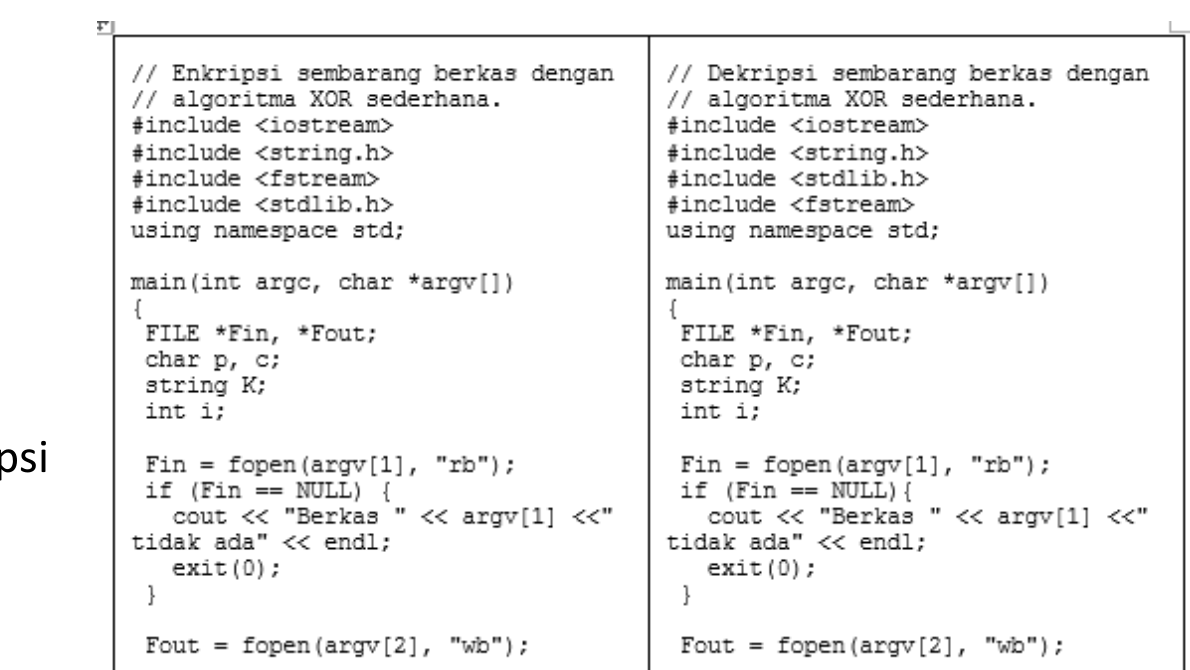
\includegraphics[width=130.20mm,height=184.14mm]{../../images/llm/page_014_img_01.png}%
\end{textblock*}

\end{document}
